\subsection{Elevation Scan}
We performed an elevation scan from the horizon \SI{10}{\degree} to the zenith \SI{90}{\degree} at different  azimuth angles.
We chose an angular step size of \SI{0.25}{\degree}. This step size was chosen as a compromise between measurement time and angular resolution.
For these measurements we made sure that the sun does not cross the scan path.
One set of measurements was performed at night (07.10.2025 21:50 - 22:20 MESZ) and the other during the day (08.10.2025 11:30 - 11:50 MESZ).

Recorded Data:

\begin{itemize}
    \item \path{Measurements/ElevationScan/ElevationScan_T2150_Az90_20251007.hdf}
    \item \path{Measurements/ElevationScan/ElevationScan_T2205_Az180_20251007.hdf}
    \item \path{Measurements/ElevationScan/2ndScanAtDay_noMilkyWay/ElevationScan_T1135_Az90_20251008.hdf}
    \item \path{Measurements/ElevationScan/2ndScanAtDay_noMilkyWay/ElevationScan_T1100_Az180_20251008_use_lower_half_idx.hdf}
\end{itemize}

As we are performing only a qualitative analysis, we do not discuss measurement errors here. We observe that the signal is stronger at low elevations for both day and night scans. Additionally, during the night, the signal increases toward the zenith, consistent with the Milky Way being near the zenith at the time of observation.
The periodic behavior seen at low elevations, which shows no phase offset across azimuth angles, is likely caused by sidelobes picking up ground interference.

\begin{figure}[H]
\centering
\begin{subfigure}[t]{0.45\textwidth}
    \centering
    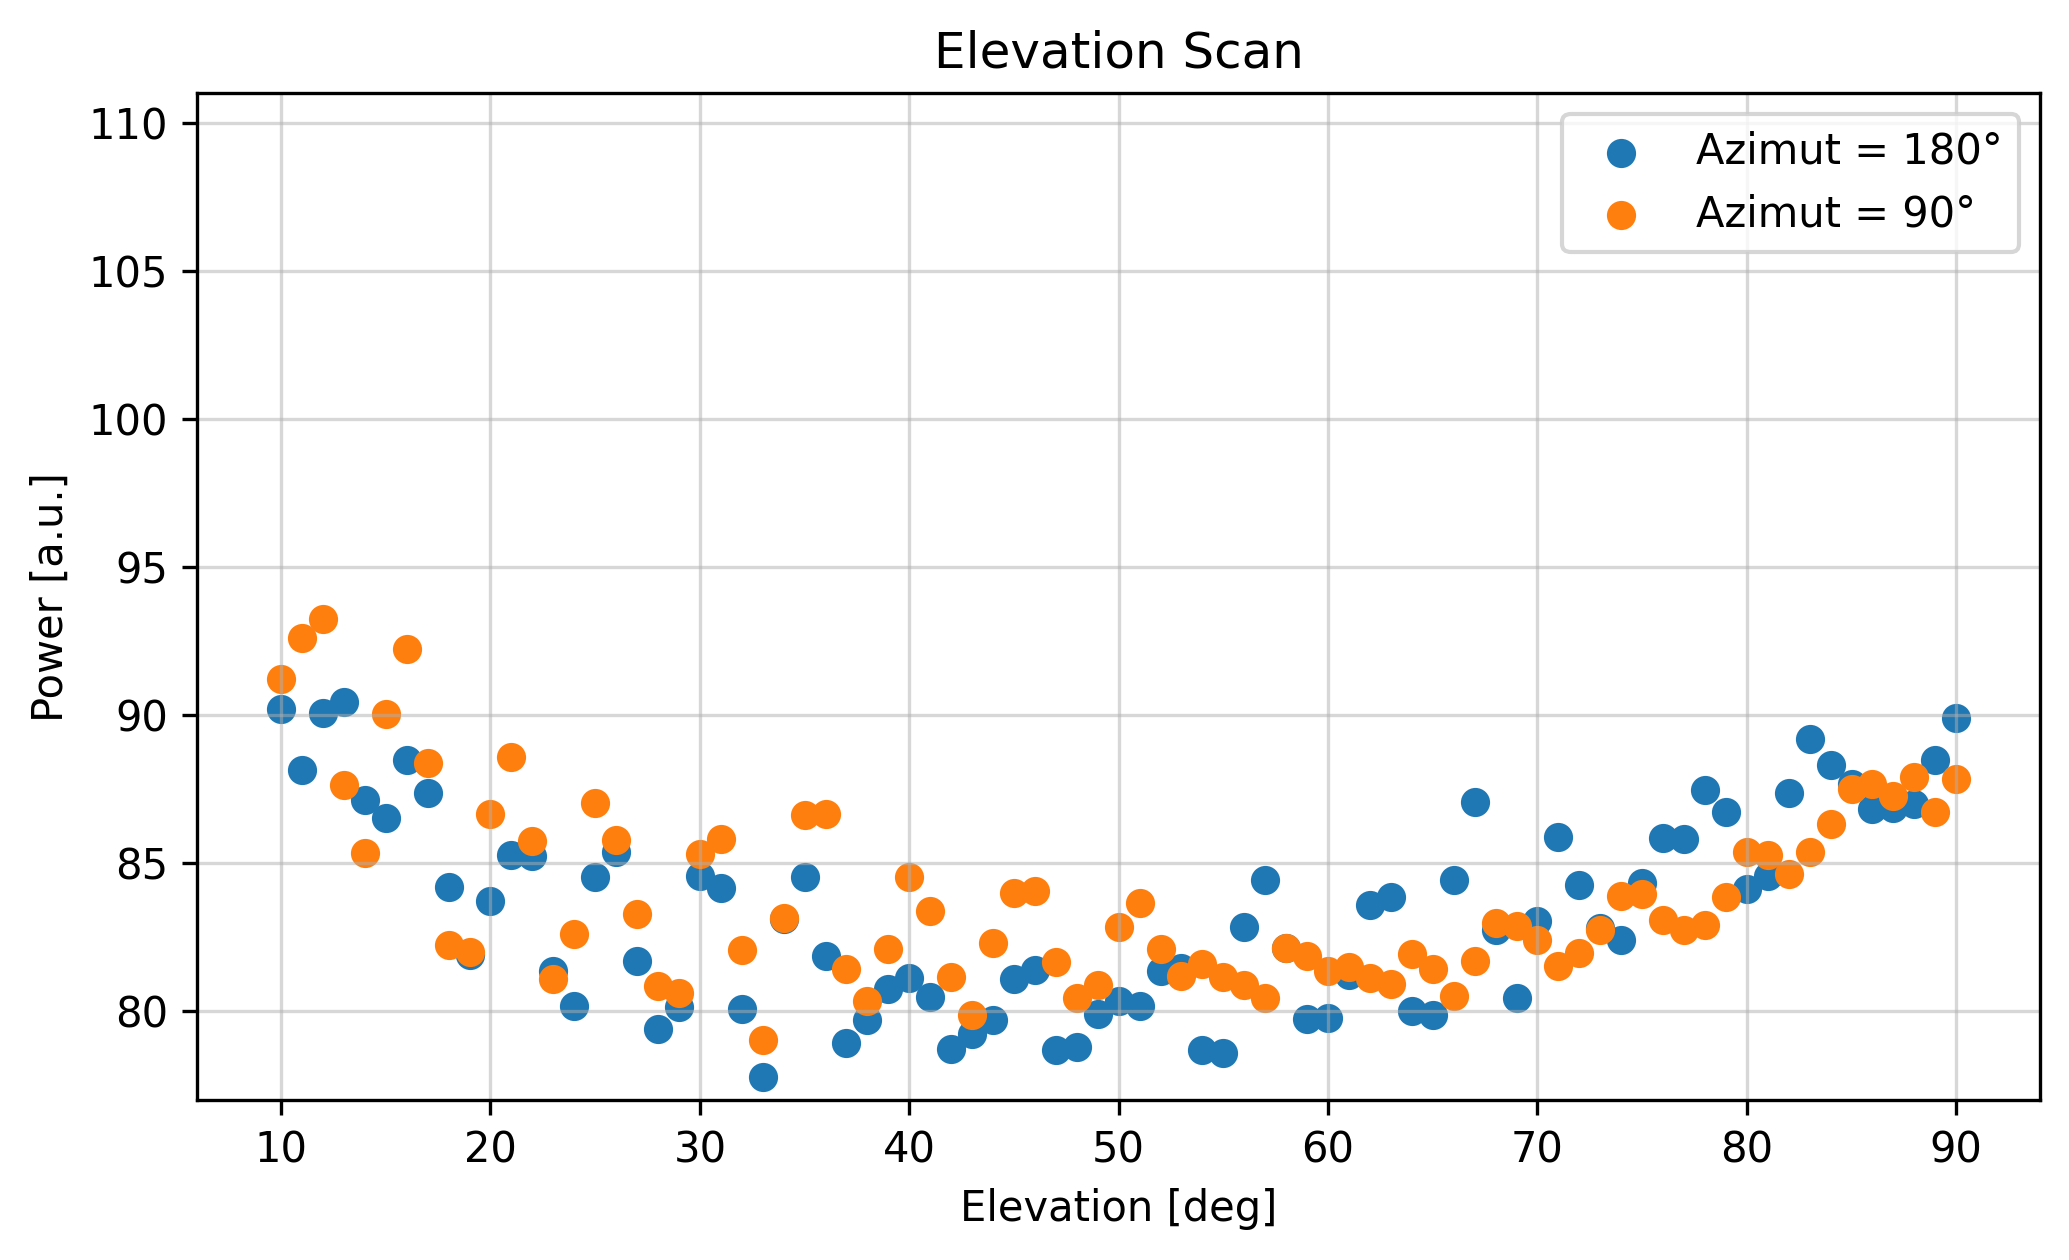
\includegraphics[width=\linewidth]{assets/elev_scan_night.png}
    \caption{Elevation Scan night}
\end{subfigure}
\begin{subfigure}[t]{0.45\textwidth}
    \centering
    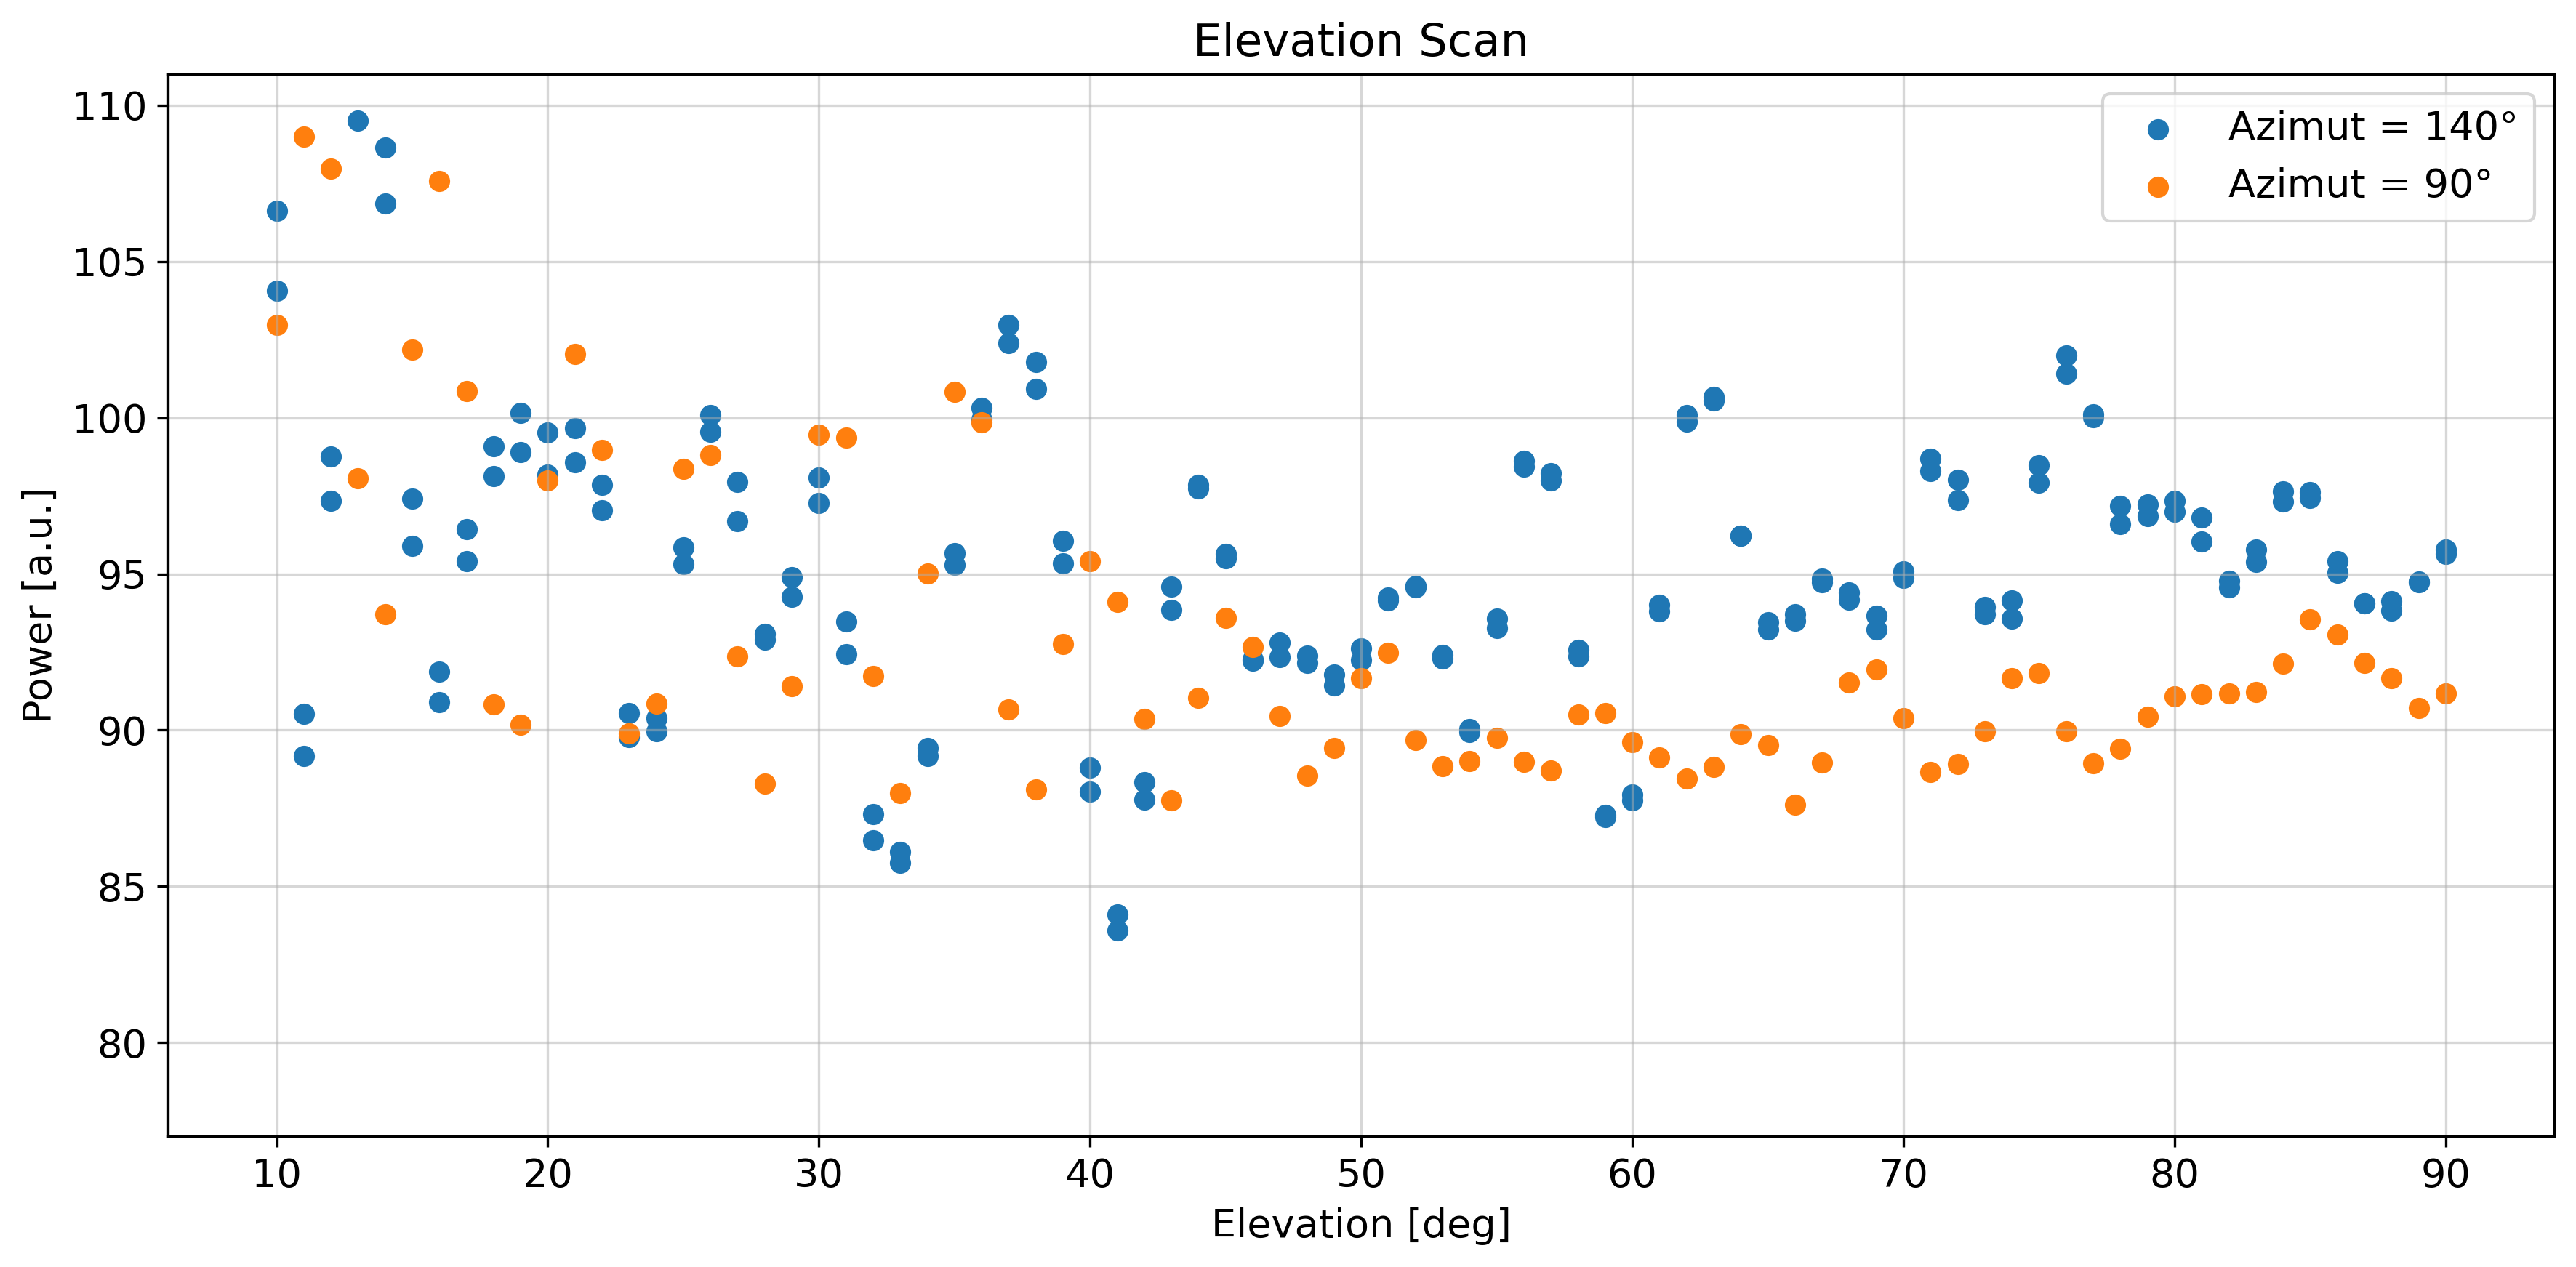
\includegraphics[width=\linewidth]{assets/elev_scan_day.png}
    \caption{Elevation Scan day}
\end{subfigure}
\caption{Elevation Scans at different times of the day}
\label{fig:elev_scan}
\end{figure}